\documentclass[]{article}
\usepackage{lmodern}
\usepackage{amssymb,amsmath}
\usepackage{ifxetex,ifluatex}
\usepackage{fixltx2e} % provides \textsubscript
\ifnum 0\ifxetex 1\fi\ifluatex 1\fi=0 % if pdftex
  \usepackage[T1]{fontenc}
  \usepackage[utf8]{inputenc}
\else % if luatex or xelatex
  \ifxetex
    \usepackage{mathspec}
  \else
    \usepackage{fontspec}
  \fi
  \defaultfontfeatures{Ligatures=TeX,Scale=MatchLowercase}
\fi
% use upquote if available, for straight quotes in verbatim environments
\IfFileExists{upquote.sty}{\usepackage{upquote}}{}
% use microtype if available
\IfFileExists{microtype.sty}{%
\usepackage{microtype}
\UseMicrotypeSet[protrusion]{basicmath} % disable protrusion for tt fonts
}{}
\usepackage[left=3.5cm,right=3.5cm,top=2cm,bottom=2cm]{geometry}
\usepackage{hyperref}
\hypersetup{unicode=true,
            pdftitle={Hands-on Machine Learning with R},
            pdfborder={0 0 0},
            breaklinks=true}
\urlstyle{same}  % don't use monospace font for urls
\usepackage{color}
\usepackage{fancyvrb}
\newcommand{\VerbBar}{|}
\newcommand{\VERB}{\Verb[commandchars=\\\{\}]}
\DefineVerbatimEnvironment{Highlighting}{Verbatim}{commandchars=\\\{\}}
% Add ',fontsize=\small' for more characters per line
\usepackage{framed}
\definecolor{shadecolor}{RGB}{248,248,248}
\newenvironment{Shaded}{\begin{snugshade}}{\end{snugshade}}
\newcommand{\AlertTok}[1]{\textcolor[rgb]{0.94,0.16,0.16}{#1}}
\newcommand{\AnnotationTok}[1]{\textcolor[rgb]{0.56,0.35,0.01}{\textbf{\textit{#1}}}}
\newcommand{\AttributeTok}[1]{\textcolor[rgb]{0.77,0.63,0.00}{#1}}
\newcommand{\BaseNTok}[1]{\textcolor[rgb]{0.00,0.00,0.81}{#1}}
\newcommand{\BuiltInTok}[1]{#1}
\newcommand{\CharTok}[1]{\textcolor[rgb]{0.31,0.60,0.02}{#1}}
\newcommand{\CommentTok}[1]{\textcolor[rgb]{0.56,0.35,0.01}{\textit{#1}}}
\newcommand{\CommentVarTok}[1]{\textcolor[rgb]{0.56,0.35,0.01}{\textbf{\textit{#1}}}}
\newcommand{\ConstantTok}[1]{\textcolor[rgb]{0.00,0.00,0.00}{#1}}
\newcommand{\ControlFlowTok}[1]{\textcolor[rgb]{0.13,0.29,0.53}{\textbf{#1}}}
\newcommand{\DataTypeTok}[1]{\textcolor[rgb]{0.13,0.29,0.53}{#1}}
\newcommand{\DecValTok}[1]{\textcolor[rgb]{0.00,0.00,0.81}{#1}}
\newcommand{\DocumentationTok}[1]{\textcolor[rgb]{0.56,0.35,0.01}{\textbf{\textit{#1}}}}
\newcommand{\ErrorTok}[1]{\textcolor[rgb]{0.64,0.00,0.00}{\textbf{#1}}}
\newcommand{\ExtensionTok}[1]{#1}
\newcommand{\FloatTok}[1]{\textcolor[rgb]{0.00,0.00,0.81}{#1}}
\newcommand{\FunctionTok}[1]{\textcolor[rgb]{0.00,0.00,0.00}{#1}}
\newcommand{\ImportTok}[1]{#1}
\newcommand{\InformationTok}[1]{\textcolor[rgb]{0.56,0.35,0.01}{\textbf{\textit{#1}}}}
\newcommand{\KeywordTok}[1]{\textcolor[rgb]{0.13,0.29,0.53}{\textbf{#1}}}
\newcommand{\NormalTok}[1]{#1}
\newcommand{\OperatorTok}[1]{\textcolor[rgb]{0.81,0.36,0.00}{\textbf{#1}}}
\newcommand{\OtherTok}[1]{\textcolor[rgb]{0.56,0.35,0.01}{#1}}
\newcommand{\PreprocessorTok}[1]{\textcolor[rgb]{0.56,0.35,0.01}{\textit{#1}}}
\newcommand{\RegionMarkerTok}[1]{#1}
\newcommand{\SpecialCharTok}[1]{\textcolor[rgb]{0.00,0.00,0.00}{#1}}
\newcommand{\SpecialStringTok}[1]{\textcolor[rgb]{0.31,0.60,0.02}{#1}}
\newcommand{\StringTok}[1]{\textcolor[rgb]{0.31,0.60,0.02}{#1}}
\newcommand{\VariableTok}[1]{\textcolor[rgb]{0.00,0.00,0.00}{#1}}
\newcommand{\VerbatimStringTok}[1]{\textcolor[rgb]{0.31,0.60,0.02}{#1}}
\newcommand{\WarningTok}[1]{\textcolor[rgb]{0.56,0.35,0.01}{\textbf{\textit{#1}}}}
\usepackage{graphicx,grffile}
\makeatletter
\def\maxwidth{\ifdim\Gin@nat@width>\linewidth\linewidth\else\Gin@nat@width\fi}
\def\maxheight{\ifdim\Gin@nat@height>\textheight\textheight\else\Gin@nat@height\fi}
\makeatother
% Scale images if necessary, so that they will not overflow the page
% margins by default, and it is still possible to overwrite the defaults
% using explicit options in \includegraphics[width, height, ...]{}
\setkeys{Gin}{width=\maxwidth,height=\maxheight,keepaspectratio}
\IfFileExists{parskip.sty}{%
\usepackage{parskip}
}{% else
\setlength{\parindent}{0pt}
\setlength{\parskip}{6pt plus 2pt minus 1pt}
}
\setlength{\emergencystretch}{3em}  % prevent overfull lines
\providecommand{\tightlist}{%
  \setlength{\itemsep}{0pt}\setlength{\parskip}{0pt}}
\setcounter{secnumdepth}{0}
% Redefines (sub)paragraphs to behave more like sections
\ifx\paragraph\undefined\else
\let\oldparagraph\paragraph
\renewcommand{\paragraph}[1]{\oldparagraph{#1}\mbox{}}
\fi
\ifx\subparagraph\undefined\else
\let\oldsubparagraph\subparagraph
\renewcommand{\subparagraph}[1]{\oldsubparagraph{#1}\mbox{}}
\fi

%%% Use protect on footnotes to avoid problems with footnotes in titles
\let\rmarkdownfootnote\footnote%
\def\footnote{\protect\rmarkdownfootnote}

%%% Change title format to be more compact
\usepackage{titling}

% Create subtitle command for use in maketitle
\providecommand{\subtitle}[1]{
  \posttitle{
    \begin{center}\large#1\end{center}
    }
}

\setlength{\droptitle}{-2em}

  \title{Hands-on Machine Learning with R}
    \pretitle{\vspace{\droptitle}\centering\huge}
  \posttitle{\par}
    \author{}
    \preauthor{}\postauthor{}
    \date{}
    \predate{}\postdate{}
  

\begin{document}
\maketitle

\setcounter{section}{3}

\hypertarget{linear-regression}{%
\section{Linear Regression}\label{linear-regression}}

\emph{Linear regression} is one of the simplest algs for supervised
learning. But it's a good starting point and many more complex methods
can be seen as extensions of it.

\hypertarget{prerequisites}{%
\subsection{Prerequisites}\label{prerequisites}}

Adding \texttt{vip} packages for interpretability of variable
importance. Ames data set from before.

\hypertarget{simple-linear-regresison}{%
\subsection{Simple Linear Regresison}\label{simple-linear-regresison}}

SLR assumes the relationship between two continuous variables is at
least approximately linear.

\[Y_i=\beta_0+\beta_1 X_i+\epsilon_i, \qquad for \quad i=1,2,...,n,\]
Where \(Y_i\) represents the response/target variable, \(X_i\) is the
\(i^{th}\) feature value and teh betas are fixed but unknown constants
(coefficients or parameters), representing the intercept and the slope.

The \(\epsilon_i\) term represents noise or random error. Here we assume
the errors have a mean of zero and constant variance \(\sigma^2\). This
is denoted as \(\stackrel{iid}{\sim}N(0, \sigma^2)\). Since the errors
are centered on zero - the expected value \(E(\epsilon_i) = 0\), linear
regression is really a problem of estimating the conditional mean:

\[E(Y_i|X_i) = \beta_0+\beta_1 X_i\] WHich we can shorten to just
\(E(Y)\). So the interpretation is in therms of \emph{average
responses}. E.g. \(\beta_0\) is the average response value when \(X=0\)
- sometimes referred to as the \emph{bias term} and \(\beta_1\) is the
increase in the average response if \(X\) increases by one unit, aka the
\emph{rate of change}.

\hypertarget{estimation}{%
\subsubsection{Estimation}\label{estimation}}

We want the best fitting line, but what is the best fit? The most common
way, called \emph{Oridnary least squares} (OLS) is to minimise the
\emph{residual sum of squares}:

\[RSS(\beta_0,\beta_1)=\sum^{n}_{i=1}[Y_i-(\beta_0+\beta_1X_i)]^2=\sum^{n}_{i=1}(Y_i-\beta_0-\beta_1X_i)^2.\]
We denote the OLS stimates of the coefficients as \(\hat \beta_0\) and
\(\hat \beta_1\). Once we have the estimated regression equation, we can
predict values of \(Y\) for \(X_{new}\):

\[\hat Y_{new} = \hat \beta_0 + \hat \beta_1 X_{new}\] Where
\(\hat Y_{new}\) is the estimated mean response at \(X = X_{new}\).

So let's try modelling the ames data relationship between the sale price
and the above ground living area.
\href{https://drsimonj.svbtle.com/visualising-residuals}{This link)}has
good info on visualising residuals.

\begin{Shaded}
\begin{Highlighting}[]
\NormalTok{model1 <{-}}\StringTok{ }\KeywordTok{lm}\NormalTok{(Sale\_Price }\OperatorTok{\textasciitilde{}}\NormalTok{Gr\_Liv\_Area, }\DataTypeTok{data =}\NormalTok{ ames\_train)}

\CommentTok{\# let\textquotesingle{}s have a look at the resisiduals and plot them }

\NormalTok{x <{-}}\StringTok{ }\NormalTok{ames\_train}
\NormalTok{x}\OperatorTok{$}\NormalTok{predicted <{-}}\StringTok{ }\KeywordTok{predict}\NormalTok{(model1)   }\CommentTok{\# Save the predicted values}
\NormalTok{x}\OperatorTok{$}\NormalTok{residuals <{-}}\StringTok{ }\KeywordTok{residuals}\NormalTok{(model1) }

\CommentTok{\# this is what the data looks like}
\NormalTok{x }\OperatorTok{\%>\%}\StringTok{ }\KeywordTok{select}\NormalTok{(Sale\_Price, predicted, residuals) }\OperatorTok{\%>\%}\StringTok{ }\KeywordTok{head}\NormalTok{()}
\end{Highlighting}
\end{Shaded}

\begin{verbatim}
## # A tibble: 6 x 3
##   Sale_Price predicted residuals
##        <int>     <dbl>     <dbl>
## 1     215000   198968.    16032.
## 2     105000   111662.    -6662.
## 3     172000   161403.    10597.
## 4     195500   192994.     2506.
## 5     213500   162437.    51063.
## 6     236500   194373.    42127.
\end{verbatim}

\begin{Shaded}
\begin{Highlighting}[]
\CommentTok{\# here are some plots}
\KeywordTok{par}\NormalTok{(}\DataTypeTok{mfrow =} \KeywordTok{c}\NormalTok{(}\DecValTok{1}\NormalTok{,}\DecValTok{2}\NormalTok{))}
\KeywordTok{par}\NormalTok{(}\DataTypeTok{mar =} \KeywordTok{c}\NormalTok{(}\DecValTok{4}\NormalTok{,}\DecValTok{4}\NormalTok{,}\DecValTok{2}\NormalTok{,}\FloatTok{0.1}\NormalTok{)}\OperatorTok{+}\FloatTok{0.10}\NormalTok{)}
\KeywordTok{plot}\NormalTok{(x}\OperatorTok{$}\NormalTok{Gr\_Liv\_Area, x}\OperatorTok{$}\NormalTok{Sale\_Price, }\DataTypeTok{col =} \KeywordTok{alpha}\NormalTok{(}\StringTok{"black"}\NormalTok{, }\FloatTok{0.3}\NormalTok{), }\DataTypeTok{pch =} \DecValTok{20}\NormalTok{,}
     \DataTypeTok{main =} \StringTok{"fitted regression line"}\NormalTok{)}
\KeywordTok{abline}\NormalTok{(model1, }\DataTypeTok{col =} \StringTok{"cadetblue4"}\NormalTok{, }\DataTypeTok{lwd =} \DecValTok{2}\NormalTok{)}
\KeywordTok{plot}\NormalTok{(x}\OperatorTok{$}\NormalTok{Gr\_Liv\_Area, x}\OperatorTok{$}\NormalTok{Sale\_Price, }\DataTypeTok{col =} \KeywordTok{alpha}\NormalTok{(}\StringTok{"black"}\NormalTok{, }\FloatTok{0.3}\NormalTok{), }\DataTypeTok{pch =} \DecValTok{20}\NormalTok{,}
     \DataTypeTok{main =} \StringTok{"fitted regression line with residuals"}\NormalTok{)}
\KeywordTok{abline}\NormalTok{(model1, }\DataTypeTok{col =} \StringTok{"cadetblue4"}\NormalTok{, }\DataTypeTok{lwd =} \DecValTok{2}\NormalTok{)}
\ControlFlowTok{for}\NormalTok{ (i }\ControlFlowTok{in} \DecValTok{1}\OperatorTok{:}\StringTok{ }\KeywordTok{nrow}\NormalTok{(x))\{}
\KeywordTok{lines}\NormalTok{(}\KeywordTok{c}\NormalTok{(x}\OperatorTok{$}\NormalTok{Gr\_Liv\_Area[i], x}\OperatorTok{$}\NormalTok{Gr\_Liv\_Area[i]),}
      \KeywordTok{c}\NormalTok{(x}\OperatorTok{$}\NormalTok{Sale\_Price[i], x}\OperatorTok{$}\NormalTok{predicted[i]), }
      \DataTypeTok{lwd =} \FloatTok{0.5}\NormalTok{)\}}
\end{Highlighting}
\end{Shaded}

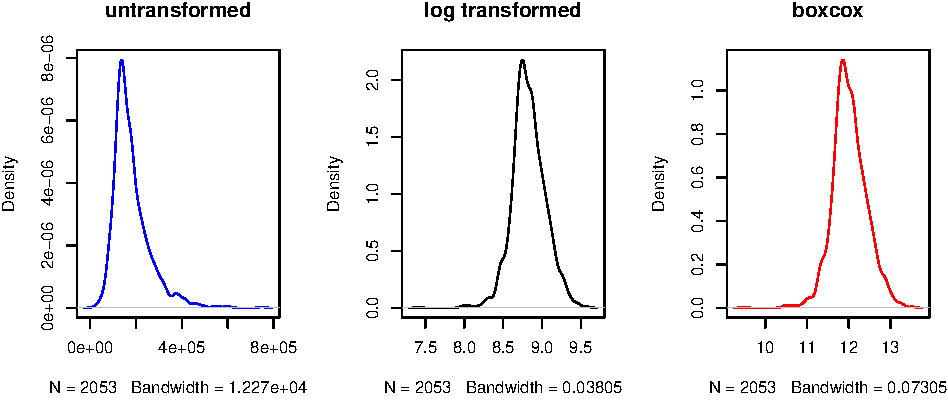
\includegraphics{ch-04-linear_regression_files/figure-latex/unnamed-chunk-2-1.pdf}

Use \texttt{coef()} and \texttt{summary()} to have a look a the
coefficients. !!! I don't get the same data, even though i have the same
seed in the split?

\begin{Shaded}
\begin{Highlighting}[]
\KeywordTok{coef}\NormalTok{(model1)}
\end{Highlighting}
\end{Shaded}

\begin{verbatim}
## (Intercept) Gr_Liv_Area 
##    8732.938     114.876
\end{verbatim}

\begin{Shaded}
\begin{Highlighting}[]
\KeywordTok{summary}\NormalTok{(model1)}
\end{Highlighting}
\end{Shaded}

\begin{verbatim}
## 
## Call:
## lm(formula = Sale_Price ~ Gr_Liv_Area, data = ames_train)
## 
## Residuals:
##     Min      1Q  Median      3Q     Max 
## -361143  -30668   -2449   22838  331357 
## 
## Coefficients:
##             Estimate Std. Error t value Pr(>|t|)    
## (Intercept) 8732.938   3996.613   2.185    0.029 *  
## Gr_Liv_Area  114.876      2.531  45.385   <2e-16 ***
## ---
## Signif. codes:  0 '***' 0.001 '**' 0.01 '*' 0.05 '.' 0.1 ' ' 1
## 
## Residual standard error: 56700 on 2051 degrees of freedom
## Multiple R-squared:  0.5011, Adjusted R-squared:  0.5008 
## F-statistic:  2060 on 1 and 2051 DF,  p-value: < 2.2e-16
\end{verbatim}

\begin{Shaded}
\begin{Highlighting}[]
\CommentTok{\# glimpse(model1)}
\end{Highlighting}
\end{Shaded}

So we estimate that an increase in area by one square foot increases the
selling price by 114.88\$. SO nice and intuitive.

One drawback of using least squares is that we only have estimates of
the coefficients, but not of the error variance \(\sigma^2\). LS makes
no assumptions about the random errors, so we cannot estimate
\(\sigma^2\).

An alternative is to use \emph{maximum likelihood} estimation (ML) to
estimate \(\sigma^2\) -- which we need to characterise the variability
of our model. For ML we have to assume a particular distribution of the
errors, most commonly that they are normally distributed. Under these
assumptions the estimate of the error variance is

\[\hat\sigma^2=\frac{1}{n-p} \sum^n_{i=1}(Y_i-\hat Y_i)^2 = \frac{1}{n-p} \sum^n_{i=1}r_i^2\]

Where \(r_i\) is the residual of the \(i^{th}\) observation. and \(p\)
is the number of parameters or coefficients in the model.
\hat\sigma\^{}2 is also known as the mean squared error (MSE) and it's
square root is the RMSE, and you can get it out of an \texttt{lm} object
using \texttt{sigma()}

\begin{Shaded}
\begin{Highlighting}[]
\KeywordTok{sigma}\NormalTok{(model1)}
\end{Highlighting}
\end{Shaded}

\begin{verbatim}
## [1] 56704.78
\end{verbatim}

\begin{Shaded}
\begin{Highlighting}[]
\KeywordTok{sigma}\NormalTok{(model1)}\OperatorTok{\^{}}\DecValTok{2}
\end{Highlighting}
\end{Shaded}

\begin{verbatim}
## [1] 3215432370
\end{verbatim}

!!! the sigma is slightly different from the RMSE reported in the
summary, not sure why, same in book.

\hypertarget{inference}{%
\subsubsection{Inference}\label{inference}}

The coefficients are only point estimates, so that's not super useful
without a measure of variability. This is usually measured with a
\emph{standard error} (SE), the square root of it's variance. If we
assume the errors are distributed \(\stackrel{iid}{\sim}N(0, \sigma^2)\)
,then the SEs for the coefficients are simple and are expressied under
the \texttt{Std.\ Error} heading in the summary for the model.

From the SE we can also do a t-test to see if the coefficients are
statistically significantly different from zero. (!!! stantistically
significant from zero is probably wrong).

The t-statistic is simply the estimated coefficient divided by the SE,
which measures the number of standard deviations each coefficient is
away from zero. The p-values are reported in the same table.

Under these same assumptions we can also derive the confidence intervals
for the \(\beta\) coefficients. The formual is:

\[\beta_j \pm t_{1-α/2,n-p} \hat {SE}(\hat \beta_j)\]

In R you can construct them using \texttt{confitn()}

\begin{Shaded}
\begin{Highlighting}[]
\KeywordTok{confint}\NormalTok{(model1, }\DataTypeTok{level =} \FloatTok{0.95}\NormalTok{)}
\end{Highlighting}
\end{Shaded}

\begin{verbatim}
##                2.5 %     97.5 %
## (Intercept) 895.0961 16570.7805
## Gr_Liv_Area 109.9121   119.8399
\end{verbatim}

\begin{Shaded}
\begin{Highlighting}[]
\CommentTok{\# or if you wanna spell it out:}
\KeywordTok{coef}\NormalTok{(model1)[}\DecValTok{2}\NormalTok{] }\OperatorTok{{-}}\StringTok{ }\KeywordTok{qt}\NormalTok{(}\FloatTok{0.975}\NormalTok{, model1}\OperatorTok{$}\NormalTok{df.residual)}\OperatorTok{*}\KeywordTok{coef}\NormalTok{(}\KeywordTok{summary}\NormalTok{(model1))[}\DecValTok{2}\NormalTok{,}\DecValTok{2}\NormalTok{]}
\end{Highlighting}
\end{Shaded}

\begin{verbatim}
## Gr_Liv_Area 
##    109.9121
\end{verbatim}

\begin{Shaded}
\begin{Highlighting}[]
\KeywordTok{coef}\NormalTok{(model1)[}\DecValTok{2}\NormalTok{] }\OperatorTok{+}\StringTok{ }\KeywordTok{qt}\NormalTok{(}\FloatTok{0.975}\NormalTok{, model1}\OperatorTok{$}\NormalTok{df.residual)}\OperatorTok{*}\KeywordTok{coef}\NormalTok{(}\KeywordTok{summary}\NormalTok{(model1))[}\DecValTok{2}\NormalTok{,}\DecValTok{2}\NormalTok{]}
\end{Highlighting}
\end{Shaded}

\begin{verbatim}
## Gr_Liv_Area 
##    119.8399
\end{verbatim}

So with 95\% confidence we estimate that the mean sale price goes up
between 109 and 119\$ for each additional square foot.

Don't forget that these SEs and t-stats etc in the summary are based on
the following assumptions:

\begin{enumerate}
\def\labelenumi{\arabic{enumi}.}
\tightlist
\item
  Independent observations
\item
  The random errors have mean zero, and constant variance
\item
  The random errors are normally distributed
\end{enumerate}

If your data deviate from these assumptions, there are some remedial
actions you can take..

\hypertarget{multiple-linear-regression}{%
\subsection{Multiple linear
regression}\label{multiple-linear-regression}}

Extend the simple linear regression with more predictors to see e.g.~how
are and year built are (linearly) related to the sales price using
\emph{mulitple linear regression} (MLR).

\[Y_i=\beta_0+\beta_1 X_i+\beta_2 X_2 + \epsilon_i, \qquad for \quad i=1,2,...,n,\]

Which you do in R by using \texttt{+} to separate predictors:

\begin{Shaded}
\begin{Highlighting}[]
\NormalTok{(model2 <{-}}\StringTok{ }\KeywordTok{lm}\NormalTok{(Sale\_Price }\OperatorTok{\textasciitilde{}}\StringTok{ }\NormalTok{Gr\_Liv\_Area }\OperatorTok{+}\StringTok{ }\NormalTok{Year\_Built, }\DataTypeTok{data =}\NormalTok{ ames\_train))}
\end{Highlighting}
\end{Shaded}

\begin{verbatim}
## 
## Call:
## lm(formula = Sale_Price ~ Gr_Liv_Area + Year_Built, data = ames_train)
## 
## Coefficients:
## (Intercept)  Gr_Liv_Area   Year_Built  
##  -2.123e+06    9.918e+01    1.093e+03
\end{verbatim}

\begin{Shaded}
\begin{Highlighting}[]
\CommentTok{\# or use update}
\NormalTok{(model2 <{-}}\StringTok{ }\KeywordTok{update}\NormalTok{(model1, .}\OperatorTok{\textasciitilde{}}\NormalTok{. }\OperatorTok{+}\StringTok{ }\NormalTok{Year\_Built))}
\end{Highlighting}
\end{Shaded}

\begin{verbatim}
## 
## Call:
## lm(formula = Sale_Price ~ Gr_Liv_Area + Year_Built, data = ames_train)
## 
## Coefficients:
## (Intercept)  Gr_Liv_Area   Year_Built  
##  -2.123e+06    9.918e+01    1.093e+03
\end{verbatim}

So holding the year constant, each additional square foot of living area
increses the mean selling price by 99\$. And holding the area constant,
each additional year the home is newer by increases the mean price by
1093\$


\end{document}
